\chapter{Navier-Stokes equation -- Incompressible flow passing a step}
\label{tut:stepflowgui}

\modinfo{Directory}{FlowStepGUI}
\modinfo{Solvers}{\Idx{FlowSolve}}
\modinfo{Tools}{\Idx{ElmerGUI}}
\modinfo{Dimensions}{2D, Steady-state}


\subsection*{Case definition}

This tutorial represents the canonical step flow of viscous fluid. 
A fluid, flowing past a step (see figure~\ref{fg:struct2}), has the density
1~kg/m$�$ and viscosity 0.01~kg/ms. The velocity profile at the inlet is
defined so that $v_x=1.0$~m/s and $v_y=0.0$~m/s. At the outlet only 
the vertical component is defined, $v_y=0.0$~m/s. At all other
walls the no-slip boundary condition, $\vec{v}=0$, is applied. 

\begin{figure}[h]
\centering
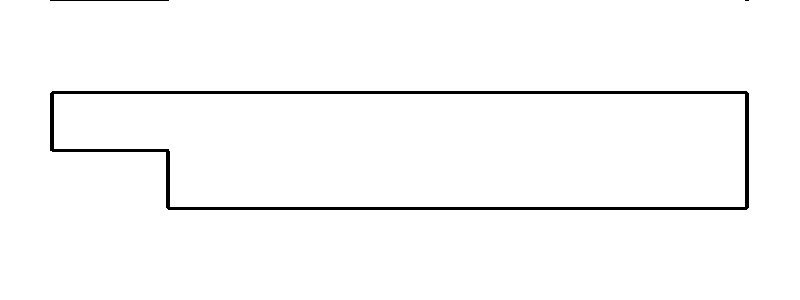
\includegraphics[width=100mm,viewport=0 30 800 270,clip]{geom}
\caption{Geometry of the step flow problem}\label{fg:struct2}
\end{figure}
%
Mathematically the problem to be solved is
\begin{equation}
\left \{
\begin{array}{rccl}
- \nabla \cdot (2 \mu \overline{\overline{\varepsilon}}) + \rho 
\vec{u} \cdot \nabla \vec{u} + \nabla p & = & 0 & \mbox{ in } \Omega \\
\nabla \cdot \vec{u} & = & 0 & \mbox{ in } \Omega \\
\end{array}
\right .
\end{equation}
%
with the boundary conditions
\begin{equation}
\left \{
\begin{array}{rccl}
u_x & = & 1 & \mbox{ on } \Gamma_{inlet} \\
u_x & = & 0 & \mbox{ on } \Gamma_{no-slip} \\
u_y & = & 0 & \mbox{ on } \Gamma_{inlet} \cup \Gamma_{outlet} \cup \Gamma_{no-slip} 
\end{array}
\right .
\end{equation}
where $\mu$ is the viscosity, $\overline{\overline{\varepsilon}}$ is 
the strain tensor,  $\rho$ is the density, $\vec{u}$ is the velocity and
$p$ is the pressure. It is assumed that the density and viscosity are 
constants. 



\subsection*{Solution procedure}

The mesh is given in ElmerGrid format in file \texttt{step.grd}, load this file.
\ttbegin
File 
  Open -> step.grd
\ttend
You should obtain your mesh and may check that it consists of 9696 nodes and of 
9442 bilinear elements.
\ttbegin
Model 
  Summary...
\ttend

After we have the mesh we start to go through the Model menu from the top to bottom. 
In the Setup we choose things related to the whole simulation.
The steady-state simulation is carried out in 2-dimensional cartesian
coordinates, which are also the defaults.  
\ttbegin
Model
  Setup 
    Simulation Type = Steady state
    Coordinate system = Cartesian
\ttend
In the equation section we choose the relevant equations and parameters related to their solution. 
In this case the only the Navier-Stokes equation is needed.

When defining Equations and Materials it is possible to assign the to bodies immediately, or to use mouse
selection to assign them later. In this case we have just one body and therefore its easier to assign 
the Equation and Material to it directly. One could also edit the solver setting in order to
try different strategies for solving the nonlinear or linear system. Initially the Navier-Stokes
solver uses the more robust Picard iteration which is changed to Newton iteration after few initial steps.
For the given viscosity the default values are ok, but may need tuning when going into higher Reynolds numbers.
\ttbegin
Model
  Equation
    Name = Navier-Stokes
    Apply to Bodies = 1
    Navier-Stokes 
      Active = on
      Edit Solver Setting
        Nonlinear System
          Max. iterations = 20
          Newton after iterations = 3
    Add 
    OK
\ttend        

The Material section includes all the material parameters.
They are divided to generic parameters which are direct properties of the material
without making any assumptions on the physical model, such as the density. Other properties assume
a physical law, such as viscosity. 
\ttbegin
Model
  Material
    Name = Ideal
    General 
      Density = 1.0
    Navier-Stokes 
      Viscosity = 0.01
    Apply to Bodies = 1 
    Add
    OK
\ttend

The current case does not have any body forces. Convergence should also be
obtained using the default initial condition which sets all field values to zero. 
Hence no setting for initial condition are needed. 

Only one boundary condition may be applied to each boundary and therefore all the 
different physical BCs for a boundary should be grouped together. In this case the
Temperature and Velocity. The side walls are assumed to be adiabatic.
\ttbegin
Model
  BoundaryCondition
    Name = Inlet
    Navier-Stokes 
      Velocity 1 = 1.0
      Velocity 2 = 0.0
    Add
    New

    Name = Outlet
    Navier-Stokes 
      Velocity 2 = 0.0
    Add 
    New
 
    Name = Walls
    Navier-Stokes 
      Velocity 1 = 0.0
      Velocity 2 = 0.0
    Add
\ttend   

The conditions may also be assigned to boundaries in the Boundary condition menu, or 
by clicking with the mouse. Here we use the latter approach as that spares us of the 
need to know the indexes of each boundary.
\ttbegin
Model
  Set boundary properties
    Choose Inlet -> set boundary condition Inlet
    Choose Outlet -> set boundary condition Outlet
    Choose Walls -> set boundary condition Walls
\ttend

For the execution 
ElmerSolver needs the mesh files and the command file. We have now basically defined
all the information for ElmerGUI to write the command file. After writing it we may also visually 
inspect the command file.
\ttbegin
Sif 
  Generate
  Edit -> look how your command file came out  
\ttend

Before we can execute the solver we should save the files in a directory. The project includes
all the files needed to restart the case. Create a suitable directory for the case if needed. 
\ttbegin
File 
  Save Project
\ttend

After we have successfully saved the files we may start the solver
\ttbegin
Run
  Start solver
\ttend
A convergence view automatically pops up showing relative changes of each iteration.
The problem should converge in nine iterations.
When there are some results to view we may start the postprocessor also
\ttbegin
Run
  Start postprocessor
\ttend


\subsection*{Results}

The results may be viewed using the postprocessor as shown in Figure~\ref{fg:step_velo} and~\ref{fg:step_pres}. 
One may also register specific values,
for example the pressure difference is 4.23~Pa, the minimum and maximum lateral velocities
are -0.164~m/s and 1.3709~m/s, respectively.
One special result of interest 
is the point, on the x-axis, at which the direction of the flow changes. 
In this case its position is about 6.6~m. 

\begin{figure}[h]
\centering
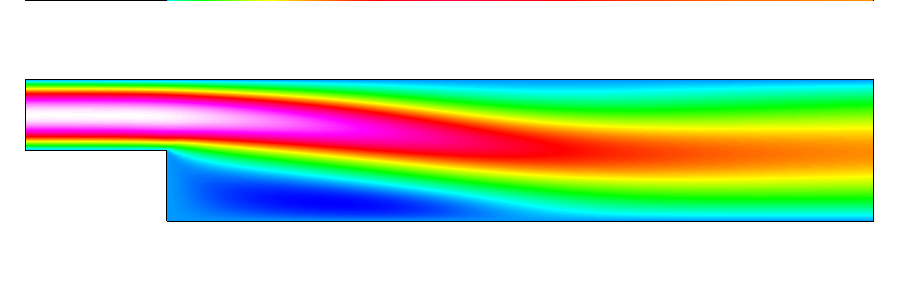
\includegraphics[width=15cm, viewport=0 30 900 270,clip]{velo_abs}
\caption{Absolute value of the velocity field}\label{fg:step_velo}
\end{figure} 

\begin{figure}[h]
\centering
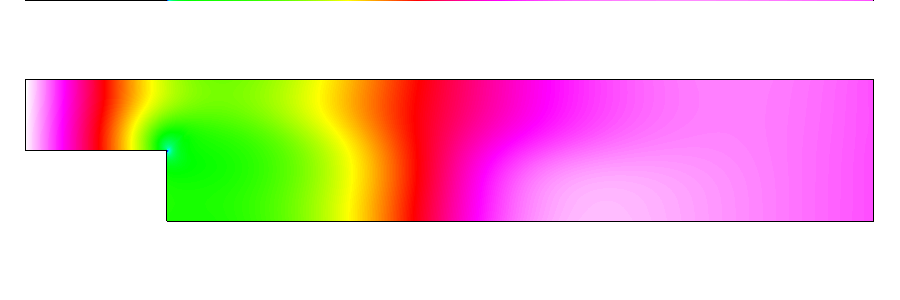
\includegraphics[width=15cm, viewport=0 30 900 270,clip]{pres}
\caption{Pressure field}\label{fg:step_pres}
\end{figure} 

   

\subsection*{Extra task: Modifying the inlet profile}

The constant inlet-profile is not very attractable. Using a analytical parabolic inlet profile 
yields better results. ElmerSolver includes MATC environment that may used to avaluate mathematical 
expressions. For that aim revisit the Boundary condition for Inlet
\ttbegin
Model
  BoundaryCondition
    Name = Inlet
    Navier-Stokes 
      Velocity 1 
\ttend
Click \texttt{Enter} to open an edit box for the \texttt{Velocity 1}. In there type the following
\ttbegin
  Variable Coordinate 2; Real MATC ``6*(tx-1)*(2-tx)''
\ttend
This expression will be interpreted at run-time so that $v_x=6(y-1)(2-y)$. As $y\in[1,2]$ this
expression creates a parabolic velocity profile with a mean velocity of unity. 
\ttbegin
    Update
    OK
\ttend

Remember to re-perform the following phases in order to get the updated results
\ttbegin
Sif 
  Generate
File 
  Save Project
Run
  Start solver
\ttend
You may just reload the results in ElmerPost rather than closing and opening the program.
It may be noted that the results have considerably changed. 


\subsection*{Extra task: Decrasing the viscosity}

Try what happens if the viscosity uis further decaresed by a factor 10. 
Convergence may be difficult to obtain. Some tricks that may be tested include
\begin{itemize}
\item Introducting a relaxation factor (typically in the range 0.5-0.7)
\item Increasing number of nonlinear iterations
\item Favoring Picard iteration over Newton 
\item Increasing mesh density (and length)
\end{itemize}



